% Options for packages loaded elsewhere
\PassOptionsToPackage{unicode}{hyperref}
\PassOptionsToPackage{hyphens}{url}
%
\documentclass[
  12pt,
  a5,margin=2cmpaper,
]{article}
\usepackage{amsmath,amssymb}
\usepackage{iftex}
\ifPDFTeX
  \usepackage[T1]{fontenc}
  \usepackage[utf8]{inputenc}
  \usepackage{textcomp} % provide euro and other symbols
\else % if luatex or xetex
  \usepackage{unicode-math} % this also loads fontspec
  \defaultfontfeatures{Scale=MatchLowercase}
  \defaultfontfeatures[\rmfamily]{Ligatures=TeX,Scale=1}
\fi
\usepackage{lmodern}
\ifPDFTeX\else
  % xetex/luatex font selection
\fi
% Use upquote if available, for straight quotes in verbatim environments
\IfFileExists{upquote.sty}{\usepackage{upquote}}{}
\IfFileExists{microtype.sty}{% use microtype if available
  \usepackage[]{microtype}
  \UseMicrotypeSet[protrusion]{basicmath} % disable protrusion for tt fonts
}{}
\makeatletter
\@ifundefined{KOMAClassName}{% if non-KOMA class
  \IfFileExists{parskip.sty}{%
    \usepackage{parskip}
  }{% else
    \setlength{\parindent}{0pt}
    \setlength{\parskip}{6pt plus 2pt minus 1pt}}
}{% if KOMA class
  \KOMAoptions{parskip=half}}
\makeatother
\usepackage{xcolor}
\usepackage{longtable,booktabs,array}
\usepackage{calc} % for calculating minipage widths
% Correct order of tables after \paragraph or \subparagraph
\usepackage{etoolbox}
\makeatletter
\patchcmd\longtable{\par}{\if@noskipsec\mbox{}\fi\par}{}{}
\makeatother
% Allow footnotes in longtable head/foot
\IfFileExists{footnotehyper.sty}{\usepackage{footnotehyper}}{\usepackage{footnote}}
\makesavenoteenv{longtable}
\usepackage{graphicx}
\makeatletter
\def\maxwidth{\ifdim\Gin@nat@width>\linewidth\linewidth\else\Gin@nat@width\fi}
\def\maxheight{\ifdim\Gin@nat@height>\textheight\textheight\else\Gin@nat@height\fi}
\makeatother
% Scale images if necessary, so that they will not overflow the page
% margins by default, and it is still possible to overwrite the defaults
% using explicit options in \includegraphics[width, height, ...]{}
\setkeys{Gin}{width=\maxwidth,height=\maxheight,keepaspectratio}
% Set default figure placement to htbp
\makeatletter
\def\fps@figure{htbp}
\makeatother
\setlength{\emergencystretch}{3em} % prevent overfull lines
\providecommand{\tightlist}{%
  \setlength{\itemsep}{0pt}\setlength{\parskip}{0pt}}
\setcounter{secnumdepth}{-\maxdimen} % remove section numbering
\newlength{\cslhangindent}
\setlength{\cslhangindent}{1.5em}
\newlength{\csllabelwidth}
\setlength{\csllabelwidth}{3em}
\newlength{\cslentryspacingunit} % times entry-spacing
\setlength{\cslentryspacingunit}{\parskip}
\newenvironment{CSLReferences}[2] % #1 hanging-ident, #2 entry spacing
 {% don't indent paragraphs
  \setlength{\parindent}{0pt}
  % turn on hanging indent if param 1 is 1
  \ifodd #1
  \let\oldpar\par
  \def\par{\hangindent=\cslhangindent\oldpar}
  \fi
  % set entry spacing
  \setlength{\parskip}{#2\cslentryspacingunit}
 }%
 {}
\usepackage{calc}
\newcommand{\CSLBlock}[1]{#1\hfill\break}
\newcommand{\CSLLeftMargin}[1]{\parbox[t]{\csllabelwidth}{#1}}
\newcommand{\CSLRightInline}[1]{\parbox[t]{\linewidth - \csllabelwidth}{#1}\break}
\newcommand{\CSLIndent}[1]{\hspace{\cslhangindent}#1}
\ifLuaTeX
  \usepackage{selnolig}  % disable illegal ligatures
\fi
\IfFileExists{bookmark.sty}{\usepackage{bookmark}}{\usepackage{hyperref}}
\IfFileExists{xurl.sty}{\usepackage{xurl}}{} % add URL line breaks if available
\urlstyle{same}
\hypersetup{
  pdftitle={Introduction},
  hidelinks,
  pdfcreator={LaTeX via pandoc}}

\title{Introduction}
\author{}
\date{}

\begin{document}
\maketitle

This thesis will focus on the most common form of prostate cancer,
prostatic adenocarcinoma. For simplicity, we will refer to this type as
just `prostate cancer.' This disease affects one in 1.4 million men
every year, making it the most prevalent common type of cancer in men
(excluding skin cancers).\textsuperscript{\textbf{Sung2021-iz?}}
Prostate cancer is a disease of the epithelial cells of the prostate.
Epithelial cells line our body cavities, hollow organs, and glands. They
undergo rapid proliferation, primarily due to damage. This proliferation
increases the risk of genetic mutations, ultimately increasing the risk
of a cell uncontrollably dividing. Together with enabling factors of its
tissue environment, this can give rise to cancer.

In general, the more aggressive cancerous cells are, the less they will
behave and morphologically appear like their original function. The
prostate is a gland that produces prostatic fluid. The fluid is
transported to the urethra by small tubes. These tubes, called prostatic
glands, are lined with epithelium. Low-grade cancer will thus mimic
those gland structures. High-grade prostate cancer loses its structural
morphology, forming sheets of cells or even quasi-randomly dispersed
individual cancerous cells.

American pathologist Donald Floyd Gleason systematically wrote down the
correlation between growth patterns and prognosis in prostate cancer in
the 1960s\textsuperscript{\textbf{cite\_original?}}. Pathologists still
use this Gleason grading, albeit several revisions
later\textsuperscript{1}, to classify prostate cancer.

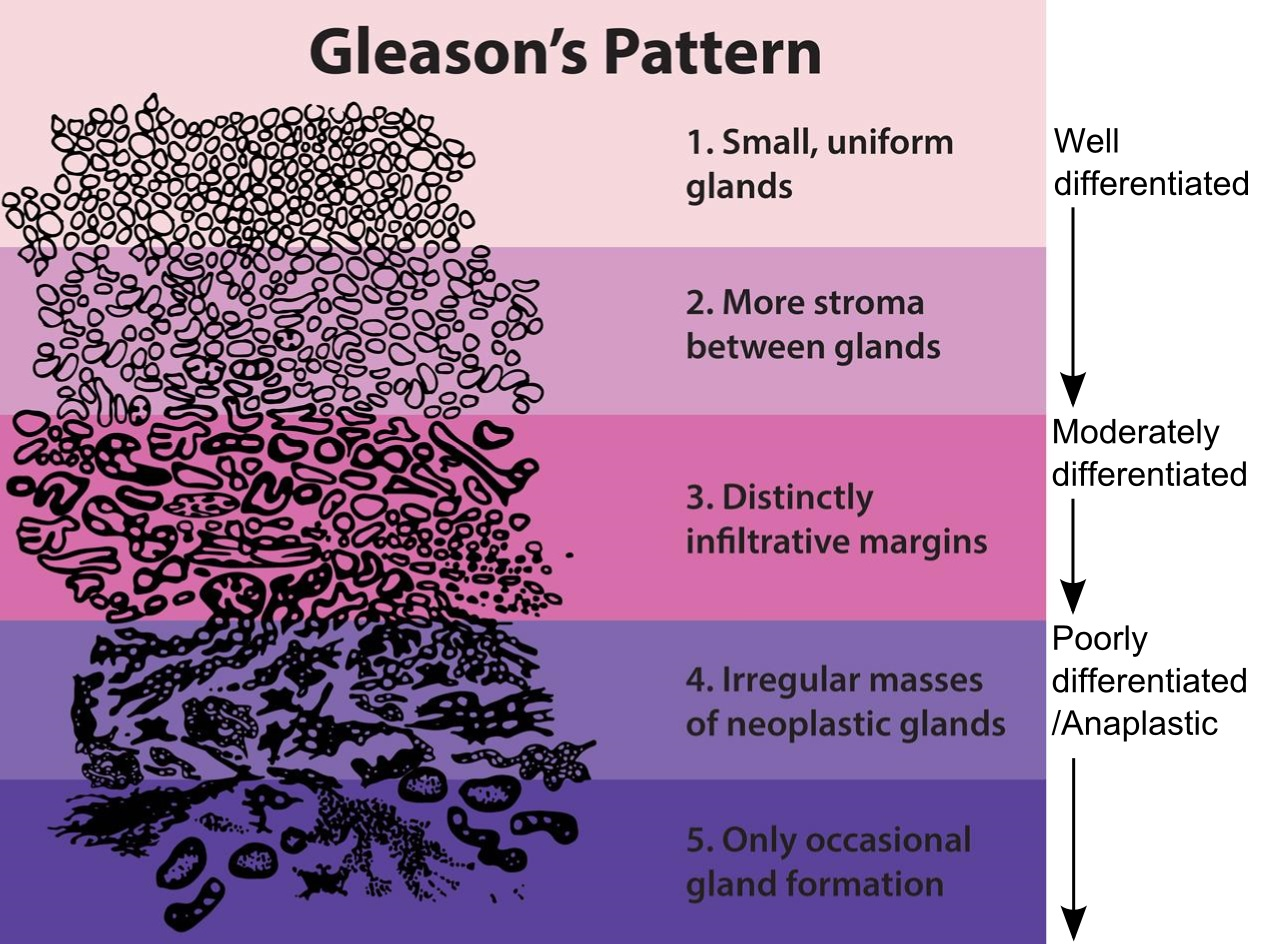
\includegraphics{chpt1_imgs/Gleasonscore.jpg}

\textbf{Gleason's growth patterns.} Image of the Gleason score for
prostate cancer grading based on the original description in 1977. From:
Morphology \& Grade. ICD-O-3 Morphology Codes. National Institutes of
Health.\textsuperscript{2}

\hypertarget{prognostic-biomarkers}{%
\section{Prognostic biomarkers}\label{prognostic-biomarkers}}

To decide on a treatment plan, clinicians divide patients into risk
groups according to traditional baseline characteristics, such as PSA
blood level, Gleason grade, tumor location, tumor size, and lymph node
status.{[}lam2019{]} This information is gathered from
histopathological, radiological assessment, and lab assessments. These
assessments can be considered biomarkers as they indicate the prognosis
of a patient\textsuperscript{3}. The more precise these assessments are,
the better we can tailor the treatment to the specific patient; this is
known as personalized medicine.

To make treatment more tailored to the patient, researchers try to
develop new biomarkers. There is a demand for new biomarkers because
most prostate cancers progress so slowly that they are unlikely to
threaten the affected individual's survival, and patients with the same
histological and clinical characteristics, can have strikingly different
outcomes\textsuperscript{4}. Being able to pick out patients with good
prognoses would improve their quality of life since treatments for
prostate cancer obviously have adverse effects
(\#tab:adverse)\{reference-type=``ref'' reference=``tab:adverse''\}).
Equally so for patients for which we can find out the treatment will not
contribute to their health. To prevent adverse effects and increase
treatment response, researchers are developing new markers in
genomics\textsuperscript{4}, radiology\textsuperscript{5}, and
pathology, the latter of which is the subject of this thesis.

\pagebreak

\hypertarget{tab:adverse}{}
\begin{longtable}[]{@{}lll@{}}
\caption{Common Prostate Cancer Treatment Options and Potential Adverse
Effects, reproduced from Dunn et al.\textsuperscript{6}}\tabularnewline
\toprule\noalign{}
\endfirsthead
\endhead
\bottomrule\noalign{}
\endlastfoot
\textbf{Treatment Option} & \textbf{Disease Progression} &
\textbf{Potential Adverse Effects} \\
Active surveillance & Localized & Illness uncertainty \\
Radical prostatectomy & Localized & Erectile dysfunction \\
& & Urinary incontinence \\
External beam radiation & Localized and advanced disease & Urinary
urgency and frequency \\
& & Dysuria, diarrhea and proctitis \\
& & Erectile dysfunction \\
& & Urinary incontinence \\
Brachytherapy & Localized & Urinary urgency and frequency \\
& & Dysuria, diarrhea and proctitis \\
& & Erectile dysfunction \\
& & Urinary incontinence \\
Cryotherapy & Localized & Erectile dysfunction \\
& & Urinary incontinence and retention \\
& & Rectal pain and fistula \\
Hormone therapy & Advanced & Fatigue \\
& & Hot flashes, and flare effect \\
& & Hyperlipidemia \\
& & Insulin resistance \\
& & Cardiovascular disease \\
& & Anemia \\
& & Osteoporosis \\
& & Erectile dysfunction \\
& & Cognitive deficits \\
Chemotherapy & Advanced & Myelosuppression \\
& & Hypersensitivity reaction \\
& & Gastrointestinal upset \\
& & Peripheral neuropathy \\
\end{longtable}

\pagebreak

\hypertarget{biomarkers-based-on-histopathology}{%
\subsection{Biomarkers based on
histopathology}\label{biomarkers-based-on-histopathology}}

We know that histopathology holds prognostic information. Commonly,
pathologists also report extra-capsular extension of the tumor and
perineural invasion, both signs of poor prognosis. As mentioned earlier,
the Gleason patterns were discovered by recording patient prognosis.
Gleason growth patterns are grouped into five different groups, of which
current pathologists mainly use the last three. It's not hard to imagine
there being more clues in the morphology of the behavior of the tumor,
if only because the landscape of prostate cancer growth patterns is
certainly more complex than the three groups we divide them into. Of
note, recently, the `subpattern' cribriform-like growth was discovered
to be an aggressive pattern.

However, these visual biomarkers are hard to explicitly specify and
quantify manually. Luckily, machine learning can help. The first chapter
will discuss this approach further. However, it makes sense to introduce
this research field, computational pathology, first.

\hypertarget{computation-pathology}{%
\subsection{Computation Pathology}\label{computation-pathology}}

Pathology is undergoing a digital revolution. More and more labs are
purchasing whole-slide scanners, with some already reading most slides
digitally. Glass slides are digitized, resulting in gigapixel digital
images, commonly referred to as whole-slide images (WSIs). Once the data
is digital, opportunities for computational analysis and assistance
arise.

Litjens et al.~{[}1{]} gave an overview of deep learning applications in
computational pathology up to 2016. Some early successes in the field
focused on segmentation, tissue classification, and disease
classification. Often reaching comparable results on the manual
performance of the tasks by pathologists. Notably, the vast majority of
these tasks are not on prognosis or treatment response prediction.
Likely due to the fact these tasks are relatively easier and the kind of
data needed is relatively cheap to obtain compared to survival data.

All state-of-the-art methods use some flavor of deep learning. A method
where we train a model with multiple layers of computations, interwoven
with non-linearities. A decade ago, optimizing these neural networks on
GPU accelerators became common. The use of GPU made us able to develop
models with a lot of layers (hence `deep' learning) on large datasets.
From the start, we have been using a type of neural network, termed
convolutional neural networks, in vision applications.

\hypertarget{convolutional-neural-networks}{%
\section{Convolutional neural
networks}\label{convolutional-neural-networks}}

Convolutional neural networks (CNNs) have emerged among the
state-of-the-art machine learning algorithms for various computer vision
tasks, such as image classification and segmentation.

The central component of a convolutional neural network is often
represented as a sliding kernel (or filter) over an input matrix,
producing an output matrix. See Figure 1. This has several advantages;
we can use a smaller kernel than the whole making the network less
complex while exploiting the fact that objects in the image are
translation invariant; a cat in the upper-left corner is still a cat in
the lower-right corner. We introduce this inductive bias to the network
by using convolutions.

\hypertarget{todo-figure-1.}{%
\paragraph{TODO: Figure 1.}\label{todo-figure-1.}}

Most convolutional neural network architectures have alternating blocks
of layers consisting of a convolutional operation, a non-linear
activation function, and often a normalization operation. The
non-linearities are essential, as they make the networks able to
represent more complex (non-linear) functions. Normalization layers
bound the output of the block to be within a specific range which helps
during the optimization of the network.

Even though sliding kernels are less complex than having one parameter
per input value, the network architectures have evolved to become deeper
and wider to enhance their accuracy further. Training larger CNNs
demands larger amounts of computer memory, which increases exponentially
with the size of input images. Consequently, most natural image datasets
in computer vision, such as ImageNet and CIFAR-10, contain sub-megapixel
images to circumvent memory limitations.

\hypertarget{todo-figure-2-about-cnns.}{%
\paragraph{TODO: Figure 2 about CNNs.}\label{todo-figure-2-about-cnns.}}

\hypertarget{todo-overview-of-a-whole-cnn}{%
\paragraph{TODO: Overview of a whole
CNN}\label{todo-overview-of-a-whole-cnn}}

In specific domains like remote sensing and medical imaging, there is a
need to train CNNs in high-resolution, where most of the information is
contained. Ideally, we want to combine the high-resolution information
with a more global context, as pathologists can do during daily
practice. However, computer memory becomes a limiting factor. The memory
requirements of CNNs increase proportionally to the input size of the
network, quickly filling up memory with multi-megapixel images. As a
result, only small CNNs can be trained with such images, rendering
state-of-the-art architectures unattainable even on large computing
clusters.

\hypertarget{weakly-supervised-methods}{%
\section{Weakly supervised methods}\label{weakly-supervised-methods}}

For others, several authors have suggested approaches to train
convolutional neural networks (CNNs) with large whole-slide images while
preventing memory bottlenecks.

The most common solution is to train on high-resolution, but smaller
regions of the slide. These patches are combined with annotations, and
this reduces the need for the whole slide to be in memory. While this
reduces the context of the whole slide down to what's contained in a
small patch, for common problems, this is context enough. For example,
tumor classification or segmentation doesn't require the context of the
whole slide.

It is possible to train with the slide-level label and patches, this
approach is called Multiple-Instance Learning. Here we assume that one
or a few patches are enough the predict the label. In a binary
classification setting, a positive slide contains at least one positive
patch and a negative slide none. Only the most informative patches per
slide are used for backpropagation. {[}cite MIL{]}

Another weakly supervised approach is to train a model to compress the
WSI into a lower-dimensional latent space. This model is often trained
on patches, in a generative or self-supervised way. This allows us to
embed the whole slide, patch-per-patch into a smaller matrix, and train
a supervised network on the compression. {[}cite NIC/CLAM{]}

There are other, even more engineering-heavy, approaches to dealing with
the high-resolution of slides. Such as using reinforcement learning,
\ldots{}

In this thesis, a novel streaming method is proposed to train CNNs
end-to-end on entire WSIs with slide-level labels. By reconstructing
activations and gradients tile-by-tile, we can develop a
memory-efficient implementation of the convolutional layers in a CNN.
This way, a CNN can learn from full contextual information at high
resolution, without relying on patches. Experiments show streaming
reaches performance on par with or improving on patch-based methods
needing more supervision. Thus, streaming enables direct learning from
morphology to aid histopathology analysis using readily available
slide-level labels.

\hypertarget{explaining-discovered-features}{%
\section{Explaining discovered
features}\label{explaining-discovered-features}}

To surface additional prognostic information in histopathology slides we
can leverage deep learning. This alone can help patients receive
better-tailored therapy. However, if we would know more about the
underlying biological processes of the cancer, we could potentially
learn how to treat the disease better in general, or even prevent it
from forming. Since deep learning finds features to perform the task at
hand, the feature space of the network can potentially offer interesting
correlations not yet discovered by scientists. This is often called a
`hypothesis-free' discovery in literature.

Besides the fact we could learn from the feature discovery of deep
learning, the fact that these networks come up with features themselves
make them less transparent than human-discovered features (such as
Gleason growth patterns). Ultimately this could make the neural network
prediction less trustworthy, because they can't be explained in common
medical terms. The field of explainable AI tries to tackle these
problems, and learnings from that field have been applied to
computational pathology.

In the beginning of the computational pathology field, researchers
investigated the feature space by visualizing the gradient signal on top
of the original image {[}gradcam, gradient saliency{]}. While it does
provide some information, it is generally quite difficult to assess what
the model has learned. Tangible information would be to surface similar
patterns across tumors of prognostic value. We would ideally show
high-level human/pathology concepts. Chapter 2 will dive into this
further.

\hypertarget{thesis-overview}{%
\section{Thesis overview}\label{thesis-overview}}

In summary, this thesis has several objectives:

\begin{quote}
``to investigate if we could develop algorithms using the entire
whole-slide images together with patient-level information.''
\end{quote}

The secondary aim of the thesis was stated as:

\begin{quote}
``to investigate if histopathology slides contain additional information
to prognosticate patient.''
\end{quote}

Chapter 2 demonstrates a deep learning system to predict the biochemical
recurrence of prostate cancer using tissue morphology. Trained on a
nested case-control study and validated on an independent cohort, the
system finds patterns predictive of recurrence beyond standard Gleason
grading. Concept-based explanations show tissue features aligned with
pathologist interpretation.

Chapter 3 proposes a method called ``streaming'' to train convolutional
neural networks end-to-end on multi-megapixel histopathology images,
circumventing memory limitations. We tile the input image and
reconstruct activations and gradients, allowing the use of entire
high-resolution images during training without cropping.

Chapter 4 applies streaming to train models on whole prostate biopsy
images using only slide-level labels from pathology reports. It shows a
modern CNN can learn from high-resolution images without patch-level
annotations. The method reaches similar performance to state-of-the-art
patch-based and multiple instance learning techniques.

Furthermore, in Chapter 5, we will show the preliminary results of
streaming on a prognostic task in the discussion.

In summary, the thesis explores computational pathology methods to
analyze entire high-resolution histopathology images despite memory
constraints. It shows neural networks can learn from morphology to aid
prostate cancer diagnosis and prognosis when trained end-to-end on
whole-slide images using readily available slide-level labels.

\pagebreak

\hypertarget{refs}{}
\begin{CSLReferences}{0}{0}
\leavevmode\vadjust pre{\hypertarget{ref-Epstein2016-im}{}}%
\CSLLeftMargin{1. }%
\CSLRightInline{Epstein JI, Egevad L, Amin MB, Delahunt B, Srigley JR,
Humphrey PA. The 2014 international society of urological pathology
({ISUP}) consensus conference on gleason grading of prostatic carcinoma.
2016;40:244-252.}

\leavevmode\vadjust pre{\hypertarget{ref-zotero-512}{}}%
\CSLLeftMargin{2. }%
\CSLRightInline{Morphology \& {Grade} \textbar{} {SEER Training}.}

\leavevmode\vadjust pre{\hypertarget{ref-chen2011}{}}%
\CSLLeftMargin{3. }%
\CSLRightInline{Chen XH, Huang S, Kerr D. Biomarkers in clinical
medicine. Published online 2011.}

\leavevmode\vadjust pre{\hypertarget{ref-cucchiara2018}{}}%
\CSLLeftMargin{4. }%
\CSLRightInline{Cucchiara V, Cooperberg MR, Dall'Era M, et al. Genomic
{Markers} in {Prostate Cancer Decision Making}. \emph{European Urology}.
2018;73(4):572-582.
doi:\href{https://doi.org/10.1016/j.eururo.2017.10.036}{10.1016/j.eururo.2017.10.036}}

\leavevmode\vadjust pre{\hypertarget{ref-roest2023}{}}%
\CSLLeftMargin{5. }%
\CSLRightInline{Roest C, Kwee TC, Saha A, Fütterer JJ, Yakar D, Huisman
H. {AI-assisted} biparametric {MRI} surveillance of prostate cancer:
Feasibility study. \emph{European Radiology}. 2023;33(1):89-96.
doi:\href{https://doi.org/10.1007/s00330-022-09032-7}{10.1007/s00330-022-09032-7}}

\leavevmode\vadjust pre{\hypertarget{ref-dunn2011}{}}%
\CSLLeftMargin{6. }%
\CSLRightInline{Dunn MW, Kazer MW. Prostate {Cancer Overview}.
\emph{Seminars in Oncology Nursing}. 2011;27(4):241-250.
doi:\href{https://doi.org/10.1016/j.soncn.2011.07.002}{10.1016/j.soncn.2011.07.002}}

\end{CSLReferences}

\end{document}
